

\section{Experimental Setup}

\subsection{Evaluation Platforms} We apply our approach to two GPU platforms.
The first platform has an NVIDIA RTX 2080Ti GPU (2080Ti), which integrates 4350 CUDA cores for floating point computation and 4350 CUDA
cores for integer operations. The GPU has 64KB of shared memory. The host machine has a 2.30GHz Intel Xeon E5-2697 CPU with 252GB memory,
running Linux kernel v4.15.0. We use CUDA Toolkit 11.0 and cuDNN 7.6.5. The second platform is an embedded GPU platform. It has an NVIDIA
Jetson AGX Xavier GPU (Xavier), which integrates 512 Volta cores and 48KB shared memory. The host machine has an 1.2GHz 8-core ARM CPU with
32GB memory, running Linux kernel v4.9.140-tegra. We use CUDA Toolkit 10.0 and cuDNN 7.6.3.


\subsection{Competing Methods} We compare our approach against cuDNN \cite{ChetlurWVCTCS14} which supports a wide range of convolution operations,
 including depthwise and pointwise convolutions optimized for GPUs.  Moreover, cuDNN can execute GEMM-, FFT- and Winograd-based convolutions, allowing
 us to compare our techniques with mainstream convolution methods. TensorFlow \cite{abadi2016tensorflow} is one of the mainstream machine learning frameworks. We also compare our approach against TensorFlow implementations of depthwise and pointwise convolutions.


\subsection{Performance Report}
We apply our approach to depthwise and pointwise convolutions of DSC.  We run each test case ten times with batch sizes of 1, 8,
16, 32, 64 and 128 on an unloaded machine and report the averaged running time. We found little variance during execution runs, less than
2\%. We run convolutions with two data types, 32-bit floating point (FP32) for normal CNNs and 8-bit integer (INT8) for quantized CNNs
\cite{nagel2019data}. In our experiments, we utilize data layouts $NCHW$ and $NHWC$ for FP32 and INT8, respectively, where $N, C, H, W$
respectively denote the batch size, the number of channels, the height and the width. CUDA \cite{cudatoolkit} provides 8-bit integer
4-element vector dot product (DP4A) instruction that performs the vector dot product between two 4-element vectors and accumulates the
result in a 32-bit integer. Utilizing the DP4A instruction, we can group four contiguous channels of the INT8 data type into a 4-element
vector to perform convolution. Therefore, we utilize $NHWC$ data layout for the INT8 data type due to its better performance over $NCHW$.

In this work, we first test depthwise convolution with two filter sizes, $3 \times 3$ and $5 \times 5$, because these are commonly used
filter sizes. Then, we report the performance of pointwise convolution. Lastly, we apply our optimized depthwise and pointwise convolutions
on the standard and quantized MobileNetV2 and EfficientNet-B0 to report the performance of both inference and training.
%
%\subsection{Notations}
%Throughout the evaluation, we use $I$, $F$, and $O$ to represent the input, the filter, and the output respectively, $N$, $C$, $H$, and $W$
%to denote the batch size, the channel, the height, and the width, respectively.

\section{Experimental Results}
\label{exp} In this section, we report results for depthwise convolution (Section \ref{sec:depconvexp}) and pointwise convolution (Section
\ref{sec:pwconvexp}), as well as inference and training of MobileNetV2 and EffcientNet-B0 (Section \ref{sec:inferexp}), showing that our approach consistently
outperforms alternative methods by delivering the overall best performance.


\subsection{Depthwise Convolution}
\label{sec:depconvexp}

\begin{table}[]
\caption{Layer configurations of depthwise  convolutions.}
\vspace{-3mm}
\label{tab:depconvconfigs}
\centering
\rowcolors{2}{}{Gray}
\begin{threeparttable}
\begin{tabular}{lrrrrr}
\toprule
\textbf{\emph{LAYER}}& \textbf{$I_N$} & \textbf{$I_C$} & \textbf{$I_H \times I_W$ }&  \textbf{$F_H \times F_W$} &\textbf{$S$}\\
\midrule
\textbf{CONV1} & 1,8,16,32,64,128  & 16    & 112$\times$112 & $3 \times 3$, $5 \times 5$&2  \\
\textbf{CONV2} & 1,8,16,32,64,128  & 72    & 56$\times$56  &$3 \times 3$, $5 \times 5$  &2 \\
\textbf{CONV3} & 1,8,16,32,64,128  & 88   & 28$\times$28  &$3 \times 3$, $5 \times 5$   &1 \\
\textbf{CONV4} & 1,8,16,32,64,128  & 96    & 28$\times$28  &$3 \times 3$, $5 \times 5$  &2  \\
\textbf{CONV5} & 1,8,16,32,64,128  & 96   & 14$\times$14  &$3 \times 3$, $5 \times 5$   &1 \\
\textbf{CONV6} & 1,8,16,32,64,128  & 120   & 14$\times$14  &$3 \times 3$, $5 \times 5$  &1  \\
\textbf{CONV7} & 1,8,16,32,64,128  & 192   & 14$\times$14  &$3 \times 3$, $5 \times 5$  &1  \\
\textbf{CONV8} & 1,8,16,32,64,128  & 240   & 14$\times$14  &$3 \times 3$, $5 \times 5$  &2  \\
\textbf{CONV9} & 1,8,16,32,64,128  & 432   & 7$\times$7  &$3 \times 3$, $5 \times 5$    &1\\

\bottomrule
\end{tabular}
\end{threeparttable}

\end{table}

\begin{figure*}[!t]
\centering
\subfloat[Speedups on 2080Ti for the $3 \times 3$ fitler.]{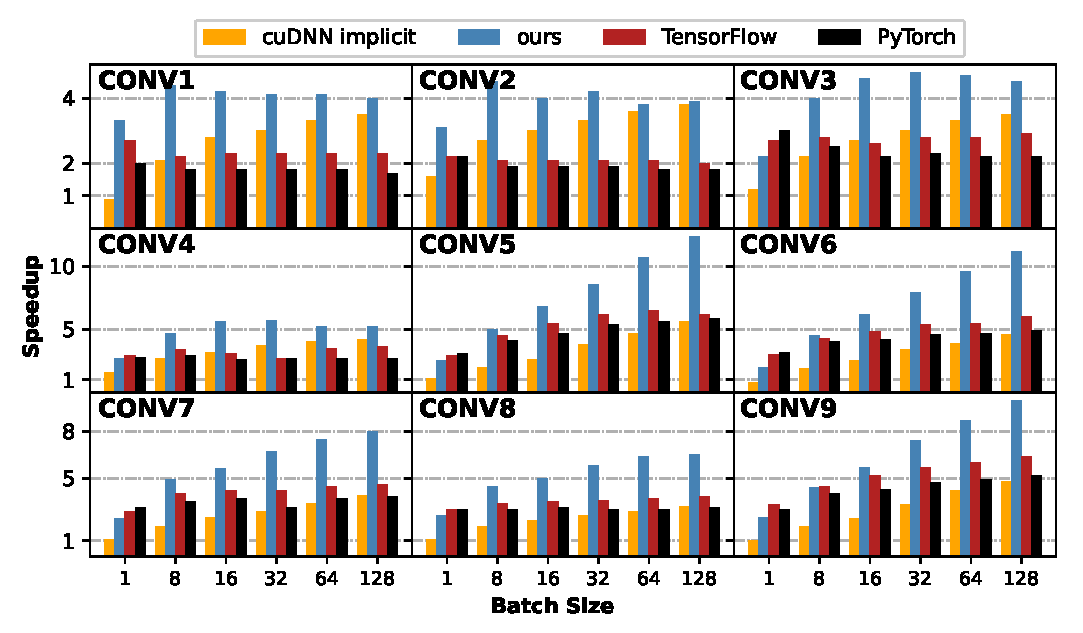
\includegraphics[height=5.12cm]{./figure/dwspeedupf3rtx.eps}
	\label{fig:dwspeeduprtxf3}}
\hspace{0em}
\subfloat[Speedups on 2080Ti for the $5 \times 5$ fitler.]{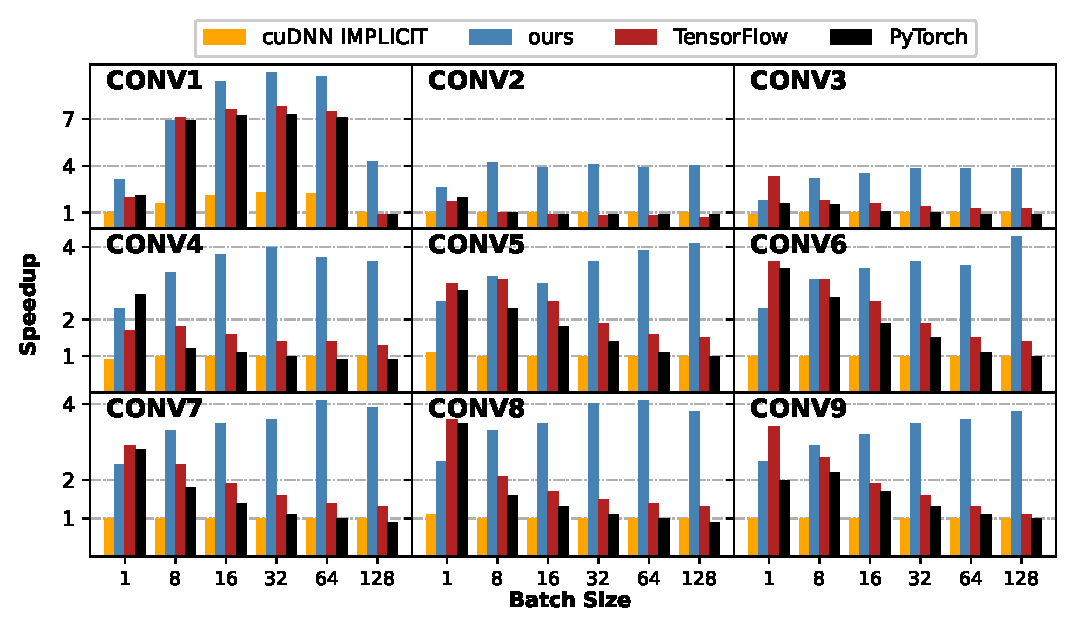
\includegraphics[height=5.12cm]{./figure/dwspeedupf5rtx.eps}
	\label{fig:dwspeeduprtxf5}}
\hspace{0em}
\subfloat[Speedups on Xavier for the $3 \times 3$ fitler.]{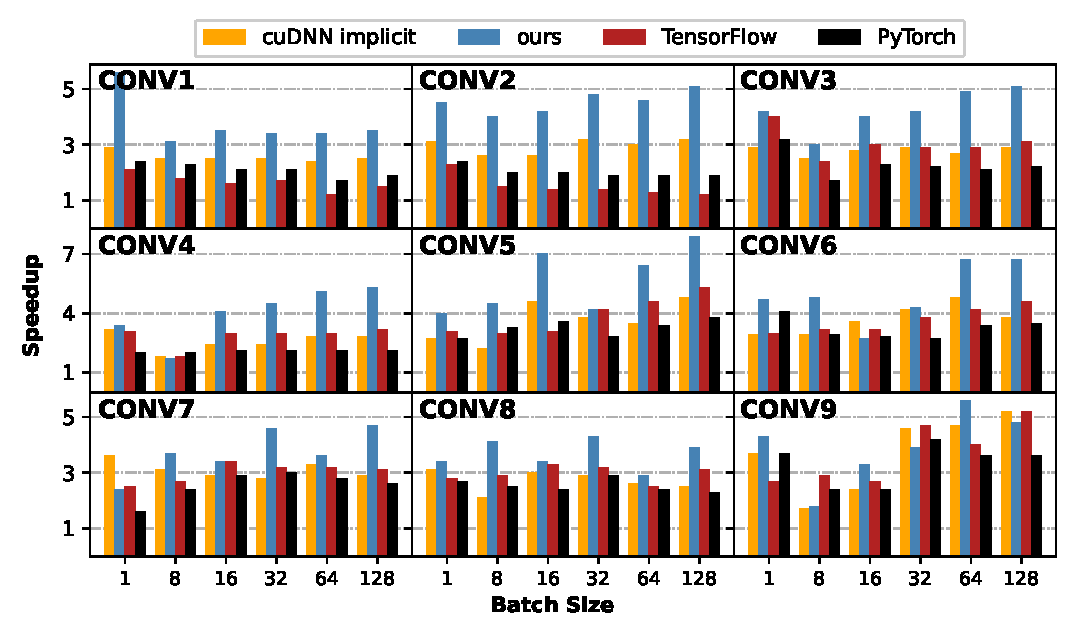
\includegraphics[height=5.12cm]{./figure/dwspeedupf3jetson.eps}
	\label{fig:dwspeedupjetsonf3}}
\hspace{0em}
\subfloat[Speedups on Xavier for the $5 \times 5$ fitler.]{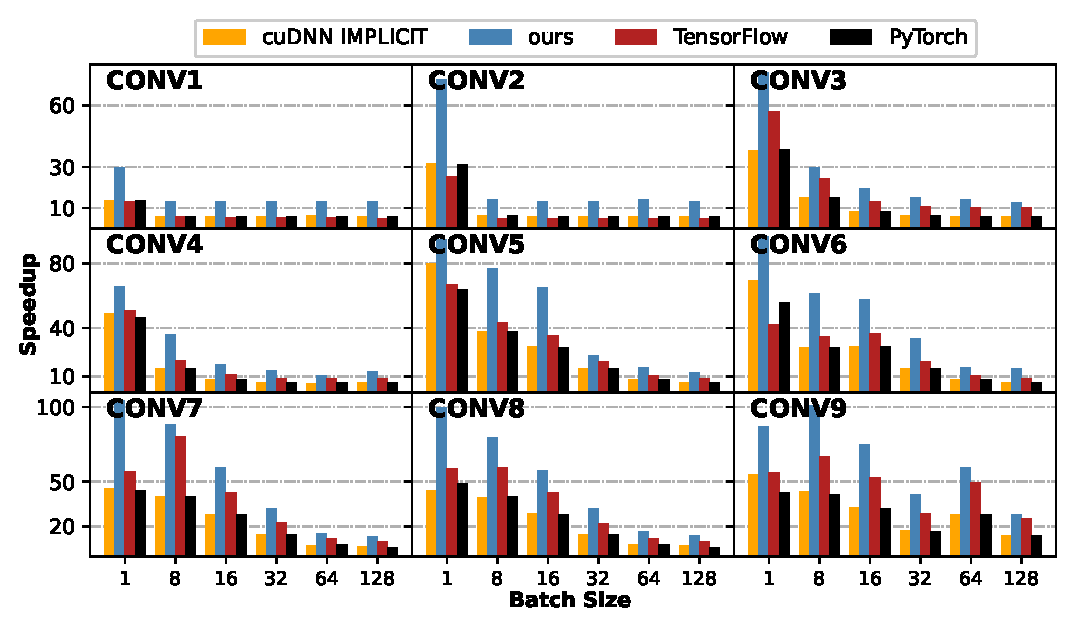
\includegraphics[height=5.12cm]{./figure/dwspeedupf5jetson.eps}
	\label{fig:dwspeedupjetsonf5}}
\caption{\RV{Speedups of IMPLICIT, PRECOMP, our approach and TensorFlow over the baseline implementation (GEMM) for FP32 depthwise convolution with filters of size $3 \times 3$ and $5 \times 5$ on two platforms.}} \label{fig:dwspeedup}
\end{figure*}



\subsubsection{Setup} In this experiment, we compare our approach against the depthwise convolution implementations of cuDNN and TensorFlow.
During the experiments, we have compared our approach to seven algorithms in cuDNN, including IMPLICIT\_GEMM (IMPLICIT), IMPLICIT\_PRECOMP\_GEMM (PRECOMP), GEMM, FFT, FFT\_TILING (TILING), WINOGRAD and WINOGRAD\_NONFUSED (NONFUSED). We found IMPLICIT and PRECOMP give the best performance \RV{in all our test cases. We report the results by comparing our approach against IMPLICIT, PRECOMP and TensorFlow, and take GEMM as the baseline in this evaluation.} Table \ref{tab:depconvconfigs} gives the layer configurations used in this experiment where the notations were defined earlier in Section \ref{sec:roadmap}.


\subsubsection{Overall results}
\mypara{FP32 implementation.} Fig. \ref{fig:dwspeedup} shows that our approach gives the best speedup in nearly all test cases. \RV{Table \ref{tab:dwspeedups} presents average speedups of IMPLICIT, PRECOMP, our approach and TensorFlow over GEMM for $3 \times 3$ and $5 \times 5$ filter sizes on 2080Ti and Xavier.}
 
\begin{table}[]
\setlength{\tabcolsep}{2.3pt}
\caption{\RV{Average speedups of four depthwise convolution implementations with FP32 over GEMM.}}
\vspace{-3mm}
\label{tab:dwspeedups}
\centering
\rowcolors{2}{}{Gray}
\begin{threeparttable}
\begin{tabular}{l|r|r|r|r}
\toprule
& $3 \times 3$, 2080Ti & $3 \times 3$, Xavier &$5 \times 5$, 2080Ti&$5 \times 5$, Xavier\\
\midrule
IMPLICIT & 1.1 & 32.8 & 1.1 & 20.0\\
PRECOMP & 1.1 & 1.2 & 1.0 & 1.4\\
ours & 2.2 & 42.8 & 3.9 &39.4 \\
TensorFlow & 1.8 & 34.6 & 2.2 & 25.3\\

\bottomrule
\end{tabular}
\end{threeparttable}
\end{table}

\RV{PRECOMP and GEMM algorithms need extra memory operations to compute output elements. Consequently, both algorithms are not suitable for depthwise convolution. TensorFlow achieves better speedups than IMPLICIT because it employs several specially designed kernels to increase the GPU utilization for different input sizes. However, both TensorFlow and IMPLICIT do not optimize memory performance for depthwise convolution. Compared to TensorFlow, our approach achieves an average speedup of $1.5 \times$ and $1.6 \times$ when using a $3 \times 3$ filter on 2080Ti and Xavier respectively, and $2.2 \times$ and $1.7 \times$ when using a $5 \times 5$ filter on 2080Ti and Xavier respectively. Since IMPLICIT is closed source, we analyze its performance through CUDA Nsight Compute \cite{nsightcompute} and present the results in Section \ref{sec:dwfurther}. Overall, our approach improves IMPLICIT by $2.0\times$ and $1.4\times$ when using a $3 \times 3$ filter on 2080Ti and Xavier respectively, and $3.5\times$ and $2.1\times$ when using a $5 \times 5$ filter on 2080Ti and Xavier respectively.}

\mypara{INT8 implementation.} We found using FP32 gives a speedup of more than $10\times$ over the INT8 version for depthwise convolution
in cuDNN. This is because the INT8 version has the overhead of dequantization (i.e., converting the results from INT8 to FP32 after
convolution) and can not fully utilize DP4A instruction to accelerate INT8 convolution. \RV{We note that TensorFlow does not optimize depthwise convolution on INT8. Nonetheless, our approach gives over $10\times$ speedups when using INT8 over cuDNN and TensorFlow.}


\subsubsection{Further analysis\label{sec:dwfurther}}

\begin{figure}[t!]
    \centering
    \subfloat[][SM utilizations of IMPLICIT and our approach.]{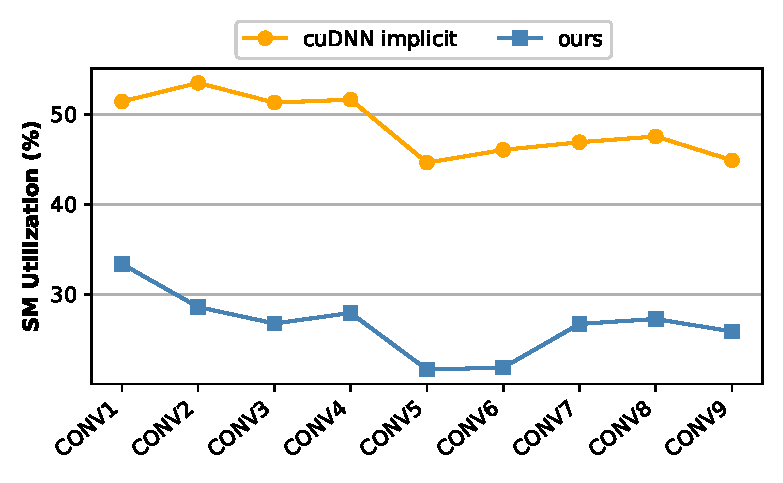
\includegraphics[width=0.9\columnwidth]{./figure/smutil.eps}\label{fig:dwsmutil}}
    \qquad
    %\vspace{5mm}
    \subfloat[][The ratio of executed LDG (load from global memory) instruction counts given by IMPLICIT over our
    approach ($ratio=\frac{LDG\ inst\ counts\ of\ cuDNN}{LDG\ inst\ counts\ of\
    ours}$).]{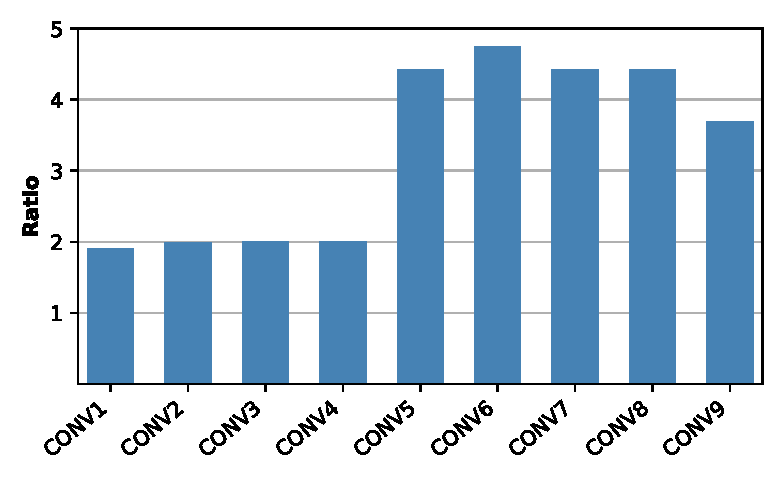
\includegraphics[width=0.9\columnwidth]{./figure/ldginst.eps}\label{fig:dwldginst}} \vspace{-2mm} \caption{SM utilizations and ratios of
    executed LDG instruction counts for depthwise convolutions with a batch size of 32 and a filter size of $3\times3$ on the NVIDIA 2080Ti GPU.}
    \label{fig:dwratio}
\end{figure}
Our performance gain is mainly attributed to the reduced number of memory accesses offered by our column and row reuse algorithms.

Fig. \ref{fig:dwratio} reports the measured LDG (load from global memory) instruction counts and SM utilization for the fast IMPLICIT algorithm and our approach when using a $3 \times 3$ filter and a batch size of 32 on 2080Ti. Other configurations follow a similar
performance trend. We can see in Fig. \ref{fig:dwsmutil} that the IMPLICIT algorithm has an average of $2\times$ higher SM
utilization compared to our approach. The reason our approach leads to lower SM utilization is explained as follows. Our row reuse
algorithm performs better when a thread operates on more rows of the output. However, the more rows a thread computes on, the fewer warps
and thread blocks we can generate. Without enough warps running on SMs, the SM utilization will degrade. Though IMPLICIT has high SM
utilization, it does not result in good performance for depthwise convolution. The reason is that depthwise convolution possesses a low
computational requirement and is more sensitive to memory performance; hence the focus of performance optimization should be reducing the
memory access latency.  If we now look at Fig. \ref{fig:dwldginst}, we see that row and column reuse techniques reduce memory operations
with up to $4.5\times$ lower LDG instructions to be executed when compared to  IMPLICIT. By reducing the memory access overhead, which
dominates the execution time of depthwise convolution, our approach thus can lead to better overall performance compared to cuDNN, despite
lower SM utilization.

\RV{From Fig. \ref{fig:dwspeedup} we can observe that speedups of our approach over IMPLICIT fluctuate in a small range as batch size increases. Both IMPLICIT and our approach can not benefit from higher GPU utilization because depthwise convolution is memory bound, thus IMPLICIT and our approach grow at the same rate.}

\subsubsection{Summary}
By reducing the number of memory accesses, our approach leads to faster memory access time and overall quick computation time when
performing depthwise convolutions. Compared to the fastest available algorithms in cuDNN, our approach achieves an average speedup of
$2.8\times$ and $1.8\times$ when performing depthwise convolutions on 2080Ti and Xavier, respectively.


\subsection{Pointwise Convolution}
\label{sec:pwconvexp}

\begin{table*}[]
\setlength{\tabcolsep}{5.5pt} \caption{\RV{Layer configurations of pointwise convolutions ($F_C=I_C$, $I_W=I_H$ and $F_W=F_H=1$)
and parameter values of $Warp_H$, $Warp_W$, $Block_{num}$ and $C_{num}$. We use the tuples ($Warp_H$, $Warp_W$, $Block_{num}$, $C_{num}$)
and [$Warp_H$, $Warp_W$, $Block_{num}$, $C_{num}$] to represent parameter values generated for 2080Ti and Xavier respectively.}}
\vspace{-3mm} \label{tab:pwconvandparas} \rowcolors{99}{}{Gray}
\begin{threeparttable}
\begin{tabular}{lrrrrrrrrrr }
\toprule
\textbf{\emph{LAYER}}& \textbf{$I_C$} & \textbf{$I_H$} & \textbf{$F_N$}& \textbf{$I_N=1$} & \textbf{$I_N=8$} &\textbf{$I_N=16$} & \textbf{$I_N=32$} &\textbf{$I_N=64$} & \textbf{$I_N=128$}\\
\midrule
\rowcolor{Gray}& & & &(\hspace{0.5em}4,\hspace{1em}12,\hspace{0.5em}2,\hspace{0.5em}\hspace{0.5em}8) &(\hspace{0.5em}4,\hspace{1em}47,\hspace{0.5em}4,\hspace{0.5em}\hspace{0.5em}2) &(\hspace{0.5em}4,\hspace{0.5em}480,\hspace{0.5em}4,\hspace{0.5em}\hspace{0.5em}1) &(\hspace{0.5em}4,\hspace{0.5em}480,\hspace{0.5em}4,\hspace{0.5em}\hspace{0.5em}1) &(\hspace{0.5em}4,\hspace{0.5em}480,\hspace{0.5em}4,\hspace{0.5em}\hspace{0.5em}1) &(\hspace{0.5em}4,1216,\hspace{0.5em}2,\hspace{0.5em}32) \\
\rowcolor{Gray}\multirow{-2}{*}{\textbf{CONV1}} &\multirow{-2}{*}{16}&\multirow{-2}{*}{$56$} & \multirow{-2}{*}{$8$}&[\hspace{0.5em}4,\hspace{1em}50,\hspace{0.5em}4,\hspace{0.5em}\hspace{0.5em}2] &[\hspace{0.5em}4,\hspace{0.5em}480,\hspace{0.5em}4,\hspace{0.5em}\hspace{0.5em}1] &[\hspace{0.5em}4,1216,\hspace{0.5em}2,\hspace{0.5em}32] &[\hspace{0.5em}4,1216,\hspace{0.5em}2,\hspace{0.5em}32] &[\hspace{0.5em}4,1216,\hspace{0.5em}2,\hspace{0.5em}32] &[\hspace{0.5em}4,1216,\hspace{0.5em}2,\hspace{0.5em}32] \\
& & & &(\hspace{0.5em}8,\hspace{1em}12,\hspace{0.5em}2,\hspace{0.5em}\hspace{0.5em}8) &(\hspace{0.5em}8,\hspace{1em}47,\hspace{0.5em}4,\hspace{0.5em}\hspace{0.5em}4) &(\hspace{0.5em}8,\hspace{0.5em}256,\hspace{0.5em}4,\hspace{0.5em}\hspace{0.5em}1) &(\hspace{0.5em}8,\hspace{0.5em}256,\hspace{0.5em}4,\hspace{0.5em}\hspace{0.5em}1) &(\hspace{0.5em}8,\hspace{0.5em}672,\hspace{0.5em}2,\hspace{0.5em}32) &(\hspace{0.5em}8,\hspace{0.5em}672,\hspace{0.5em}2,\hspace{0.5em}32) \\
\multirow{-2}{*}{\textbf{CONV2}} &\multirow{-2}{*}{8}&\multirow{-2}{*}{$56$} & \multirow{-2}{*}{$16$}&[\hspace{0.5em}8,\hspace{1em}50,\hspace{0.5em}4,\hspace{0.5em}\hspace{0.5em}4] &[\hspace{0.5em}8,\hspace{0.5em}672,\hspace{0.5em}2,\hspace{0.5em}32] &[\hspace{0.5em}8,\hspace{0.5em}672,\hspace{0.5em}2,\hspace{0.5em}32] &[\hspace{0.5em}8,\hspace{0.5em}672,\hspace{0.5em}2,\hspace{0.5em}32] &[\hspace{0.5em}8,\hspace{0.5em}672,\hspace{0.5em}2,\hspace{0.5em}32] &[\hspace{0.5em}8,\hspace{0.5em}672,\hspace{0.5em}2,\hspace{0.5em}32] \\
\rowcolor{Gray}& & & &(12,\hspace{1em}36,\hspace{0.5em}2,\hspace{0.5em}\hspace{0.5em}8) &(12,\hspace{1em}36,\hspace{0.5em}4,\hspace{0.5em}\hspace{0.5em}4) &(12,\hspace{1em}36,\hspace{0.5em}4,\hspace{0.5em}\hspace{0.5em}4) &(12,\hspace{1em}36,\hspace{0.5em}4,\hspace{0.5em}\hspace{0.5em}4) &(12,\hspace{1em}36,\hspace{0.5em}4,\hspace{0.5em}\hspace{0.5em}4) &(12,\hspace{1em}36,\hspace{0.5em}4,\hspace{0.5em}\hspace{0.5em}4) \\
\rowcolor{Gray}\multirow{-2}{*}{\textbf{CONV3}} &\multirow{-2}{*}{16}&\multirow{-2}{*}{$56$} & \multirow{-2}{*}{$72$}&[12,\hspace{1em}36,\hspace{0.5em}4,\hspace{0.5em}\hspace{0.5em}4] &[12,\hspace{1em}36,\hspace{0.5em}4,\hspace{0.5em}\hspace{0.5em}4] &[12,\hspace{1em}36,\hspace{0.5em}4,\hspace{0.5em}\hspace{0.5em}4] &[12,\hspace{1em}36,\hspace{0.5em}4,\hspace{0.5em}\hspace{0.5em}4] &[12,\hspace{1em}36,\hspace{0.5em}4,\hspace{0.5em}\hspace{0.5em}4] &[12,\hspace{1em}36,\hspace{0.5em}4,\hspace{0.5em}\hspace{0.5em}4] \\
& & & &(\hspace{0.5em}6,\hspace{1.5em}6,\hspace{0.5em}2,\hspace{0.5em}32) &(\hspace{0.5em}6,\hspace{1em}47,\hspace{0.5em}2,\hspace{0.5em}\hspace{0.5em}4) &(\hspace{0.5em}6,\hspace{1em}47,\hspace{0.5em}4,\hspace{0.5em}\hspace{0.5em}4) &(\hspace{0.5em}6,\hspace{0.5em}320,\hspace{0.5em}4,\hspace{0.5em}\hspace{0.5em}1) &(\hspace{0.5em}6,\hspace{0.5em}320,\hspace{0.5em}4,\hspace{0.5em}\hspace{0.5em}1) &(\hspace{0.5em}6,\hspace{0.5em}864,\hspace{0.5em}2,\hspace{0.5em}32) \\
\multirow{-2}{*}{\textbf{CONV4}} &\multirow{-2}{*}{72}&\multirow{-2}{*}{$28$} & \multirow{-2}{*}{$24$}&[\hspace{0.5em}6,\hspace{1em}50,\hspace{0.5em}2,\hspace{0.5em}\hspace{0.5em}4] &[\hspace{0.5em}6,\hspace{0.5em}320,\hspace{0.5em}4,\hspace{0.5em}\hspace{0.5em}1] &[\hspace{0.5em}6,\hspace{0.5em}864,\hspace{0.5em}2,\hspace{0.5em}32] &[\hspace{0.5em}6,\hspace{0.5em}864,\hspace{0.5em}2,\hspace{0.5em}32] &[\hspace{0.5em}6,\hspace{0.5em}864,\hspace{0.5em}2,\hspace{0.5em}32] &[\hspace{0.5em}6,\hspace{0.5em}864,\hspace{0.5em}2,\hspace{0.5em}32] \\
\rowcolor{Gray}& & & &(\hspace{0.5em}3,\hspace{1em}48,\hspace{0.5em}2,\hspace{0.5em}\hspace{0.5em}2) &(12,\hspace{1em}48,\hspace{0.5em}4,\hspace{0.5em}\hspace{0.5em}2) &(12,\hspace{1em}48,\hspace{0.5em}4,\hspace{0.5em}\hspace{0.5em}2) &(12,\hspace{1em}48,\hspace{0.5em}4,\hspace{0.5em}\hspace{0.5em}2) &(12,\hspace{1em}48,\hspace{0.5em}4,\hspace{0.5em}\hspace{0.5em}2) &(12,\hspace{1em}48,\hspace{0.5em}4,\hspace{0.5em}\hspace{0.5em}2) \\
\rowcolor{Gray}\multirow{-2}{*}{\textbf{CONV5}} &\multirow{-2}{*}{24}&\multirow{-2}{*}{$28$} & \multirow{-2}{*}{$96$}&[12,\hspace{1em}48,\hspace{0.5em}4,\hspace{0.5em}\hspace{0.5em}2] &[12,\hspace{1em}48,\hspace{0.5em}4,\hspace{0.5em}\hspace{0.5em}2] &[12,\hspace{1em}48,\hspace{0.5em}4,\hspace{0.5em}\hspace{0.5em}2] &[12,\hspace{1em}48,\hspace{0.5em}4,\hspace{0.5em}\hspace{0.5em}2] &[12,\hspace{1em}48,\hspace{0.5em}4,\hspace{0.5em}\hspace{0.5em}2] &[12,\hspace{1em}48,\hspace{0.5em}4,\hspace{0.5em}\hspace{0.5em}2] \\
& & & &(\hspace{0.5em}6,\hspace{1.5em}2,\hspace{0.5em}2,\hspace{0.5em}32) &(\hspace{0.5em}6,\hspace{1em}12,\hspace{0.5em}2,\hspace{0.5em}16) &(\hspace{0.5em}6,\hspace{1em}24,\hspace{0.5em}2,\hspace{0.5em}\hspace{0.5em}8) &(\hspace{0.5em}6,\hspace{1em}47,\hspace{0.5em}2,\hspace{0.5em}\hspace{0.5em}4) &(\hspace{0.5em}6,\hspace{1em}47,\hspace{0.5em}4,\hspace{0.5em}\hspace{0.5em}4) &(\hspace{0.5em}6,\hspace{0.5em}320,\hspace{0.5em}4,\hspace{0.5em}\hspace{0.5em}1) \\
\multirow{-2}{*}{\textbf{CONV6}} &\multirow{-2}{*}{96}&\multirow{-2}{*}{$14$} & \multirow{-2}{*}{$24$}&[\hspace{0.5em}6,\hspace{1em}13,\hspace{0.5em}2,\hspace{0.5em}16] &[\hspace{0.5em}6,\hspace{1em}50,\hspace{0.5em}4,\hspace{0.5em}\hspace{0.5em}4] &[\hspace{0.5em}6,\hspace{0.5em}320,\hspace{0.5em}4,\hspace{0.5em}\hspace{0.5em}1] &[\hspace{0.5em}6,\hspace{0.5em}320,\hspace{0.5em}4,\hspace{0.5em}\hspace{0.5em}1] &[\hspace{0.5em}6,\hspace{0.5em}864,\hspace{0.5em}2,\hspace{0.5em}32] &[\hspace{0.5em}6,\hspace{0.5em}864,\hspace{0.5em}2,\hspace{0.5em}32] \\
\rowcolor{Gray}& & & &(\hspace{0.5em}2,\hspace{1em}48,\hspace{0.5em}2,\hspace{0.5em}\hspace{0.5em}1) &(\hspace{0.5em}6,\hspace{1em}48,\hspace{0.5em}2,\hspace{0.5em}\hspace{0.5em}4) &(12,\hspace{1em}48,\hspace{0.5em}2,\hspace{0.5em}\hspace{0.5em}8) &(12,\hspace{1em}48,\hspace{0.5em}4,\hspace{0.5em}\hspace{0.5em}2) &(12,\hspace{1em}48,\hspace{0.5em}4,\hspace{0.5em}\hspace{0.5em}2) &(12,\hspace{1em}48,\hspace{0.5em}4,\hspace{0.5em}\hspace{0.5em}2) \\
\rowcolor{Gray}\multirow{-2}{*}{\textbf{CONV7}} &\multirow{-2}{*}{24}&\multirow{-2}{*}{$14$} & \multirow{-2}{*}{$96$}&[\hspace{0.5em}7,\hspace{1em}48,\hspace{0.5em}2,\hspace{0.5em}\hspace{0.5em}4] &[12,\hspace{1em}48,\hspace{0.5em}4,\hspace{0.5em}\hspace{0.5em}2] &[12,\hspace{1em}48,\hspace{0.5em}4,\hspace{0.5em}\hspace{0.5em}2] &[12,\hspace{1em}48,\hspace{0.5em}4,\hspace{0.5em}\hspace{0.5em}2] &[12,\hspace{1em}48,\hspace{0.5em}4,\hspace{0.5em}\hspace{0.5em}2] &[12,\hspace{1em}48,\hspace{0.5em}4,\hspace{0.5em}\hspace{0.5em}2] \\
& & & &(\hspace{0.5em}2,\hspace{1em}96,\hspace{0.5em}2,\hspace{0.5em}\hspace{0.5em}1) &(\hspace{0.5em}6,\hspace{1em}96,\hspace{0.5em}2,\hspace{0.5em}\hspace{0.5em}2) &(12,\hspace{1em}96,\hspace{0.5em}2,\hspace{0.5em}\hspace{0.5em}4) &(12,\hspace{1em}96,\hspace{0.5em}4,\hspace{0.5em}\hspace{0.5em}1) &(12,\hspace{1em}96,\hspace{0.5em}4,\hspace{0.5em}\hspace{0.5em}1) &(12,\hspace{1em}96,\hspace{0.5em}4,\hspace{0.5em}\hspace{0.5em}1) \\
\multirow{-2}{*}{\textbf{CONV8}} &\multirow{-2}{*}{32}&\multirow{-2}{*}{$14$} & \multirow{-2}{*}{$192$}&[\hspace{0.5em}7,\hspace{1em}96,\hspace{0.5em}2,\hspace{0.5em}\hspace{0.5em}2] &[12,\hspace{1em}96,\hspace{0.5em}4,\hspace{0.5em}\hspace{0.5em}1] &[12,\hspace{1em}96,\hspace{0.5em}4,\hspace{0.5em}\hspace{0.5em}1] &[12,\hspace{1em}96,\hspace{0.5em}4,\hspace{0.5em}\hspace{0.5em}1] &[12,\hspace{1em}96,\hspace{0.5em}4,\hspace{0.5em}\hspace{0.5em}1] &[12,\hspace{1em}96,\hspace{0.5em}4,\hspace{0.5em}\hspace{0.5em}1] \\
\rowcolor{Gray}& & & &(12,\hspace{1.5em}2,\hspace{0.5em}2,\hspace{0.5em}32) &(12,\hspace{1em}12,\hspace{0.5em}2,\hspace{0.5em}32) &(12,\hspace{1em}24,\hspace{0.5em}2,\hspace{0.5em}16) &(12,\hspace{1em}47,\hspace{0.5em}2,\hspace{0.5em}\hspace{0.5em}8) &(12,\hspace{1em}47,\hspace{0.5em}4,\hspace{0.5em}\hspace{0.5em}2) &(12,\hspace{0.5em}160,\hspace{0.5em}4,\hspace{0.5em}\hspace{0.5em}1) \\
\rowcolor{Gray}\multirow{-2}{*}{\textbf{CONV9}} &\multirow{-2}{*}{192}&\multirow{-2}{*}{$14$} & \multirow{-2}{*}{$48$}&[12,\hspace{1em}13,\hspace{0.5em}2,\hspace{0.5em}32] &[12,\hspace{1em}50,\hspace{0.5em}4,\hspace{0.5em}\hspace{0.5em}2] &[12,\hspace{0.5em}160,\hspace{0.5em}4,\hspace{0.5em}\hspace{0.5em}1] &[12,\hspace{0.5em}480,\hspace{0.5em}2,\hspace{0.5em}32] &[12,\hspace{0.5em}480,\hspace{0.5em}2,\hspace{0.5em}32] &[12,\hspace{0.5em}480,\hspace{0.5em}2,\hspace{0.5em}32] \\
& & & &(10,\hspace{1.5em}2,\hspace{0.5em}2,\hspace{0.5em}32) &(10,\hspace{1em}12,\hspace{0.5em}2,\hspace{0.5em}32) &(10,\hspace{1em}24,\hspace{0.5em}2,\hspace{0.5em}16) &(10,\hspace{1em}47,\hspace{0.5em}2,\hspace{0.5em}\hspace{0.5em}8) &(10,\hspace{1em}47,\hspace{0.5em}4,\hspace{0.5em}\hspace{0.5em}4) &(10,\hspace{0.5em}192,\hspace{0.5em}4,\hspace{0.5em}\hspace{0.5em}1) \\
\multirow{-2}{*}{\textbf{CONV10}} &\multirow{-2}{*}{96}&\multirow{-2}{*}{$14$} & \multirow{-2}{*}{$40$}&[10,\hspace{1em}13,\hspace{0.5em}2,\hspace{0.5em}16] &[10,\hspace{1em}50,\hspace{0.5em}4,\hspace{0.5em}\hspace{0.5em}2] &[10,\hspace{0.5em}192,\hspace{0.5em}4,\hspace{0.5em}\hspace{0.5em}1] &[10,\hspace{0.5em}544,\hspace{0.5em}2,\hspace{0.5em}32] &[10,\hspace{0.5em}544,\hspace{0.5em}2,\hspace{0.5em}32] &[10,\hspace{0.5em}544,\hspace{0.5em}2,\hspace{0.5em}32] \\
\rowcolor{Gray}& & & &(\hspace{0.5em}2,\hspace{1em}60,\hspace{0.5em}2,\hspace{0.5em}\hspace{0.5em}1) &(\hspace{0.5em}6,\hspace{1em}60,\hspace{0.5em}2,\hspace{0.5em}\hspace{0.5em}2) &(12,\hspace{1em}60,\hspace{0.5em}2,\hspace{0.5em}\hspace{0.5em}4) &(12,\hspace{1em}60,\hspace{0.5em}4,\hspace{0.5em}\hspace{0.5em}2) &(12,\hspace{1em}60,\hspace{0.5em}4,\hspace{0.5em}\hspace{0.5em}2) &(12,\hspace{1em}60,\hspace{0.5em}4,\hspace{0.5em}\hspace{0.5em}2) \\
\rowcolor{Gray}\multirow{-2}{*}{\textbf{CONV11}} &\multirow{-2}{*}{40}&\multirow{-2}{*}{$14$} & \multirow{-2}{*}{$120$}&[\hspace{0.5em}7,\hspace{1em}60,\hspace{0.5em}2,\hspace{0.5em}\hspace{0.5em}4] &[12,\hspace{1em}60,\hspace{0.5em}4,\hspace{0.5em}\hspace{0.5em}2] &[12,\hspace{1em}60,\hspace{0.5em}4,\hspace{0.5em}\hspace{0.5em}2] &[12,\hspace{1em}60,\hspace{0.5em}4,\hspace{0.5em}\hspace{0.5em}2] &[12,\hspace{1em}60,\hspace{0.5em}4,\hspace{0.5em}\hspace{0.5em}2] &[12,\hspace{1em}60,\hspace{0.5em}4,\hspace{0.5em}\hspace{0.5em}2] \\
& & & &(\hspace{0.5em}8,\hspace{1.5em}2,\hspace{0.5em}2,\hspace{0.5em}32) &(\hspace{0.5em}8,\hspace{1em}12,\hspace{0.5em}2,\hspace{0.5em}16) &(\hspace{0.5em}8,\hspace{1em}24,\hspace{0.5em}2,\hspace{0.5em}\hspace{0.5em}8) &(\hspace{0.5em}8,\hspace{1em}47,\hspace{0.5em}2,\hspace{0.5em}\hspace{0.5em}4) &(\hspace{0.5em}8,\hspace{1em}47,\hspace{0.5em}4,\hspace{0.5em}\hspace{0.5em}4) &(\hspace{0.5em}8,\hspace{0.5em}256,\hspace{0.5em}4,\hspace{0.5em}\hspace{0.5em}1) \\
\multirow{-2}{*}{\textbf{CONV12}} &\multirow{-2}{*}{120}&\multirow{-2}{*}{$14$} & \multirow{-2}{*}{$32$}&[\hspace{0.5em}8,\hspace{1em}13,\hspace{0.5em}2,\hspace{0.5em}16] &[\hspace{0.5em}8,\hspace{1em}50,\hspace{0.5em}4,\hspace{0.5em}\hspace{0.5em}4] &[\hspace{0.5em}8,\hspace{0.5em}256,\hspace{0.5em}4,\hspace{0.5em}\hspace{0.5em}1] &[\hspace{0.5em}8,\hspace{0.5em}256,\hspace{0.5em}4,\hspace{0.5em}\hspace{0.5em}1] &[\hspace{0.5em}8,\hspace{0.5em}672,\hspace{0.5em}2,\hspace{0.5em}32] &[\hspace{0.5em}8,\hspace{0.5em}672,\hspace{0.5em}2,\hspace{0.5em}32] \\
\rowcolor{Gray}& & & &(\hspace{0.5em}2,\hspace{0.5em}120,\hspace{0.5em}2,\hspace{0.5em}\hspace{0.5em}1) &(\hspace{0.5em}6,\hspace{0.5em}120,\hspace{0.5em}2,\hspace{0.5em}\hspace{0.5em}1) &(12,\hspace{0.5em}120,\hspace{0.5em}2,\hspace{0.5em}\hspace{0.5em}4) &(12,\hspace{0.5em}120,\hspace{0.5em}4,\hspace{0.5em}\hspace{0.5em}1) &(12,\hspace{0.5em}120,\hspace{0.5em}4,\hspace{0.5em}\hspace{0.5em}1) &(12,\hspace{0.5em}120,\hspace{0.5em}4,\hspace{0.5em}\hspace{0.5em}1) \\
\rowcolor{Gray}\multirow{-2}{*}{\textbf{CONV13}} &\multirow{-2}{*}{40}&\multirow{-2}{*}{$14$} & \multirow{-2}{*}{$240$}&[\hspace{0.5em}7,\hspace{0.5em}120,\hspace{0.5em}2,\hspace{0.5em}\hspace{0.5em}2] &[12,\hspace{0.5em}120,\hspace{0.5em}4,\hspace{0.5em}\hspace{0.5em}1] &[12,\hspace{0.5em}120,\hspace{0.5em}4,\hspace{0.5em}\hspace{0.5em}1] &[12,\hspace{0.5em}120,\hspace{0.5em}4,\hspace{0.5em}\hspace{0.5em}1] &[12,\hspace{0.5em}120,\hspace{0.5em}4,\hspace{0.5em}\hspace{0.5em}1] &[12,\hspace{0.5em}120,\hspace{0.5em}4,\hspace{0.5em}\hspace{0.5em}1] \\
& & & &(\hspace{0.5em}2,\hspace{1em}32,\hspace{0.5em}2,\hspace{0.5em}\hspace{0.5em}2) &(\hspace{0.5em}2,\hspace{1em}32,\hspace{0.5em}2,\hspace{0.5em}\hspace{0.5em}2) &(\hspace{0.5em}3,\hspace{1em}32,\hspace{0.5em}2,\hspace{0.5em}\hspace{0.5em}2) &(\hspace{0.5em}6,\hspace{1em}32,\hspace{0.5em}2,\hspace{0.5em}\hspace{0.5em}4) &(12,\hspace{1em}32,\hspace{0.5em}2,\hspace{0.5em}\hspace{0.5em}8) &(12,\hspace{1em}32,\hspace{0.5em}4,\hspace{0.5em}\hspace{0.5em}4) \\
\multirow{-2}{*}{\textbf{CONV14}} &\multirow{-2}{*}{240}&\multirow{-2}{*}{$7$} & \multirow{-2}{*}{$64$}&[\hspace{0.5em}2,\hspace{1em}32,\hspace{0.5em}2,\hspace{0.5em}\hspace{0.5em}2] &[\hspace{0.5em}7,\hspace{1em}32,\hspace{0.5em}4,\hspace{0.5em}\hspace{0.5em}8] &[12,\hspace{1em}32,\hspace{0.5em}4,\hspace{0.5em}\hspace{0.5em}4] &[12,\hspace{1em}32,\hspace{0.5em}4,\hspace{0.5em}\hspace{0.5em}4] &[12,\hspace{1em}32,\hspace{0.5em}4,\hspace{0.5em}\hspace{0.5em}4] &[12,\hspace{1em}32,\hspace{0.5em}4,\hspace{0.5em}\hspace{0.5em}4] \\
\rowcolor{Gray}& & & &(\hspace{0.5em}2,\hspace{0.5em}120,\hspace{0.5em}2,\hspace{0.5em}\hspace{0.5em}1) &(\hspace{0.5em}2,\hspace{0.5em}120,\hspace{0.5em}2,\hspace{0.5em}\hspace{0.5em}1) &(\hspace{0.5em}3,\hspace{0.5em}120,\hspace{0.5em}2,\hspace{0.5em}\hspace{0.5em}1) &(\hspace{0.5em}6,\hspace{0.5em}120,\hspace{0.5em}2,\hspace{0.5em}\hspace{0.5em}1) &(12,\hspace{0.5em}120,\hspace{0.5em}2,\hspace{0.5em}\hspace{0.5em}4) &(12,\hspace{0.5em}120,\hspace{0.5em}4,\hspace{0.5em}\hspace{0.5em}1) \\
\rowcolor{Gray}\multirow{-2}{*}{\textbf{CONV15}} &\multirow{-2}{*}{64}&\multirow{-2}{*}{$7$} & \multirow{-2}{*}{$240$}&[\hspace{0.5em}2,\hspace{0.5em}120,\hspace{0.5em}2,\hspace{0.5em}\hspace{0.5em}1] &[\hspace{0.5em}7,\hspace{0.5em}120,\hspace{0.5em}4,\hspace{0.5em}\hspace{0.5em}2] &[12,\hspace{0.5em}120,\hspace{0.5em}4,\hspace{0.5em}\hspace{0.5em}1] &[12,\hspace{0.5em}120,\hspace{0.5em}4,\hspace{0.5em}\hspace{0.5em}1] &[12,\hspace{0.5em}120,\hspace{0.5em}4,\hspace{0.5em}\hspace{0.5em}1] &[12,\hspace{0.5em}120,\hspace{0.5em}4,\hspace{0.5em}\hspace{0.5em}1] \\
& & & &(\hspace{0.5em}2,\hspace{0.5em}216,\hspace{0.5em}2,\hspace{0.5em}\hspace{0.5em}1) &(\hspace{0.5em}2,\hspace{0.5em}216,\hspace{0.5em}2,\hspace{0.5em}\hspace{0.5em}1) &(\hspace{0.5em}3,\hspace{0.5em}216,\hspace{0.5em}2,\hspace{0.5em}\hspace{0.5em}1) &(\hspace{0.5em}6,\hspace{0.5em}216,\hspace{0.5em}2,\hspace{0.5em}\hspace{0.5em}1) &(12,\hspace{0.5em}216,\hspace{0.5em}2,\hspace{0.5em}\hspace{0.5em}2) &(\hspace{0.5em}9,\hspace{0.5em}216,\hspace{0.5em}4,\hspace{0.5em}32) \\
\multirow{-2}{*}{\textbf{CONV16}} &\multirow{-2}{*}{72}&\multirow{-2}{*}{$7$} & \multirow{-2}{*}{$432$}&[\hspace{0.5em}2,\hspace{0.5em}216,\hspace{0.5em}2,\hspace{0.5em}\hspace{0.5em}1] &[\hspace{0.5em}7,\hspace{0.5em}216,\hspace{0.5em}4,\hspace{0.5em}\hspace{0.5em}1] &[\hspace{0.5em}9,\hspace{0.5em}216,\hspace{0.5em}4,\hspace{0.5em}32] &[\hspace{0.5em}9,\hspace{0.5em}216,\hspace{0.5em}4,\hspace{0.5em}32] &[\hspace{0.5em}9,\hspace{0.5em}216,\hspace{0.5em}4,\hspace{0.5em}32] &[\hspace{0.5em}9,\hspace{0.5em}216,\hspace{0.5em}4,\hspace{0.5em}32] \\
\rowcolor{Gray}& & & &(\hspace{0.5em}2,\hspace{1em}56,\hspace{0.5em}2,\hspace{0.5em}\hspace{0.5em}1) &(\hspace{0.5em}2,\hspace{1em}56,\hspace{0.5em}2,\hspace{0.5em}\hspace{0.5em}1) &(\hspace{0.5em}3,\hspace{1em}56,\hspace{0.5em}2,\hspace{0.5em}\hspace{0.5em}1) &(\hspace{0.5em}6,\hspace{1em}56,\hspace{0.5em}2,\hspace{0.5em}\hspace{0.5em}4) &(12,\hspace{1em}56,\hspace{0.5em}2,\hspace{0.5em}\hspace{0.5em}8) &(12,\hspace{1em}56,\hspace{0.5em}4,\hspace{0.5em}\hspace{0.5em}2) \\
\rowcolor{Gray}\multirow{-2}{*}{\textbf{CONV17}} &\multirow{-2}{*}{432}&\multirow{-2}{*}{$7$} & \multirow{-2}{*}{$112$}&[\hspace{0.5em}2,\hspace{1em}56,\hspace{0.5em}2,\hspace{0.5em}\hspace{0.5em}1] &[\hspace{0.5em}7,\hspace{1em}56,\hspace{0.5em}4,\hspace{0.5em}\hspace{0.5em}4] &[12,\hspace{1em}56,\hspace{0.5em}4,\hspace{0.5em}\hspace{0.5em}2] &[12,\hspace{1em}56,\hspace{0.5em}4,\hspace{0.5em}\hspace{0.5em}2] &[12,\hspace{1em}56,\hspace{0.5em}4,\hspace{0.5em}\hspace{0.5em}2] &[12,\hspace{1em}56,\hspace{0.5em}4,\hspace{0.5em}\hspace{0.5em}2] \\
& & & &(\hspace{0.5em}2,\hspace{0.5em}216,\hspace{0.5em}2,\hspace{0.5em}\hspace{0.5em}1) &(\hspace{0.5em}2,\hspace{0.5em}216,\hspace{0.5em}2,\hspace{0.5em}\hspace{0.5em}1) &(\hspace{0.5em}3,\hspace{0.5em}216,\hspace{0.5em}2,\hspace{0.5em}\hspace{0.5em}1) &(\hspace{0.5em}6,\hspace{0.5em}216,\hspace{0.5em}2,\hspace{0.5em}\hspace{0.5em}1) &(12,\hspace{0.5em}216,\hspace{0.5em}2,\hspace{0.5em}\hspace{0.5em}2) &(\hspace{0.5em}9,\hspace{0.5em}216,\hspace{0.5em}4,\hspace{0.5em}32) \\
\multirow{-2}{*}{\textbf{CONV18}} &\multirow{-2}{*}{112}&\multirow{-2}{*}{$7$} & \multirow{-2}{*}{$432$}&[\hspace{0.5em}2,\hspace{0.5em}216,\hspace{0.5em}2,\hspace{0.5em}\hspace{0.5em}1] &[\hspace{0.5em}7,\hspace{0.5em}216,\hspace{0.5em}4,\hspace{0.5em}\hspace{0.5em}1] &[\hspace{0.5em}9,\hspace{0.5em}216,\hspace{0.5em}4,\hspace{0.5em}32] &[\hspace{0.5em}9,\hspace{0.5em}216,\hspace{0.5em}4,\hspace{0.5em}32] &[\hspace{0.5em}9,\hspace{0.5em}216,\hspace{0.5em}4,\hspace{0.5em}32] &[\hspace{0.5em}9,\hspace{0.5em}216,\hspace{0.5em}4,\hspace{0.5em}32] \\
\rowcolor{Gray}& & & &(\hspace{0.5em}2,\hspace{1em}36,\hspace{0.5em}2,\hspace{0.5em}\hspace{0.5em}1) &(\hspace{0.5em}2,\hspace{1em}36,\hspace{0.5em}2,\hspace{0.5em}\hspace{0.5em}1) &(\hspace{0.5em}3,\hspace{1em}36,\hspace{0.5em}2,\hspace{0.5em}\hspace{0.5em}2) &(\hspace{0.5em}6,\hspace{1em}36,\hspace{0.5em}2,\hspace{0.5em}\hspace{0.5em}4) &(12,\hspace{1em}36,\hspace{0.5em}2,\hspace{0.5em}\hspace{0.5em}8) &(12,\hspace{1em}36,\hspace{0.5em}4,\hspace{0.5em}\hspace{0.5em}4) \\
\rowcolor{Gray}\multirow{-2}{*}{\textbf{CONV19}} &\multirow{-2}{*}{432}&\multirow{-2}{*}{$7$} & \multirow{-2}{*}{$72$}&[\hspace{0.5em}2,\hspace{1em}36,\hspace{0.5em}2,\hspace{0.5em}\hspace{0.5em}1] &[\hspace{0.5em}7,\hspace{1em}36,\hspace{0.5em}4,\hspace{0.5em}\hspace{0.5em}4] &[12,\hspace{1em}36,\hspace{0.5em}4,\hspace{0.5em}\hspace{0.5em}4] &[12,\hspace{1em}36,\hspace{0.5em}4,\hspace{0.5em}\hspace{0.5em}4] &[12,\hspace{1em}36,\hspace{0.5em}4,\hspace{0.5em}\hspace{0.5em}4] &[12,\hspace{1em}36,\hspace{0.5em}4,\hspace{0.5em}\hspace{0.5em}4] \\
& & & &(\hspace{0.5em}2,\hspace{0.5em}256,\hspace{0.5em}2,\hspace{0.5em}\hspace{0.5em}1) &(\hspace{0.5em}3,\hspace{0.5em}256,\hspace{0.5em}2,\hspace{0.5em}\hspace{0.5em}1) &(\hspace{0.5em}6,\hspace{0.5em}256,\hspace{0.5em}2,\hspace{0.5em}\hspace{0.5em}1) &(12,\hspace{0.5em}256,\hspace{0.5em}2,\hspace{0.5em}\hspace{0.5em}1) &(\hspace{0.5em}8,\hspace{0.5em}256,\hspace{0.5em}4,\hspace{0.5em}32) &(\hspace{0.5em}8,\hspace{0.5em}256,\hspace{0.5em}4,\hspace{0.5em}32) \\
\multirow{-2}{*}{\textbf{CONV20}} &\multirow{-2}{*}{432}&\multirow{-2}{*}{$7$} & \multirow{-2}{*}{$1024$}&[\hspace{0.5em}4,\hspace{0.5em}256,\hspace{0.5em}2,\hspace{0.5em}\hspace{0.5em}1] &[\hspace{0.5em}8,\hspace{0.5em}256,\hspace{0.5em}4,\hspace{0.5em}32] &[\hspace{0.5em}8,\hspace{0.5em}256,\hspace{0.5em}4,\hspace{0.5em}32] &[\hspace{0.5em}8,\hspace{0.5em}256,\hspace{0.5em}4,\hspace{0.5em}32] &[\hspace{0.5em}8,\hspace{0.5em}256,\hspace{0.5em}4,\hspace{0.5em}32] &[\hspace{0.5em}8,\hspace{0.5em}256,\hspace{0.5em}4,\hspace{0.5em}32] \\
\bottomrule
\end{tabular}
\end{threeparttable}
\end{table*}




\begin{figure*}
\captionsetup[subfloat]{labelformat=empty,skip=0pt}
	\centering
	\subfloat[]{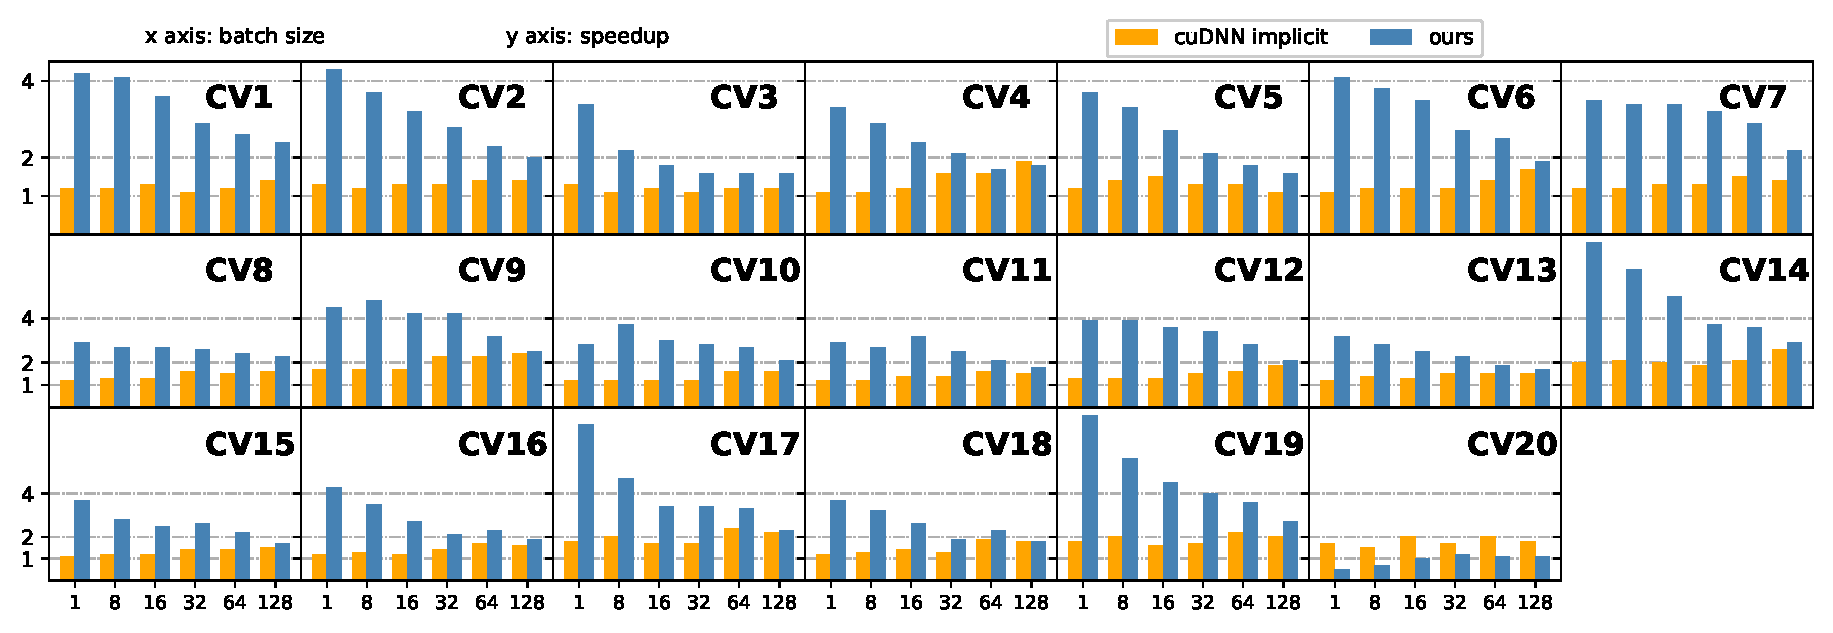
\includegraphics[width=\textwidth]{./figure/pwspeeduprtx.eps}
	\label{fig:pwspeeduprtx}}
\vspace{-5mm}
	\subfloat[]{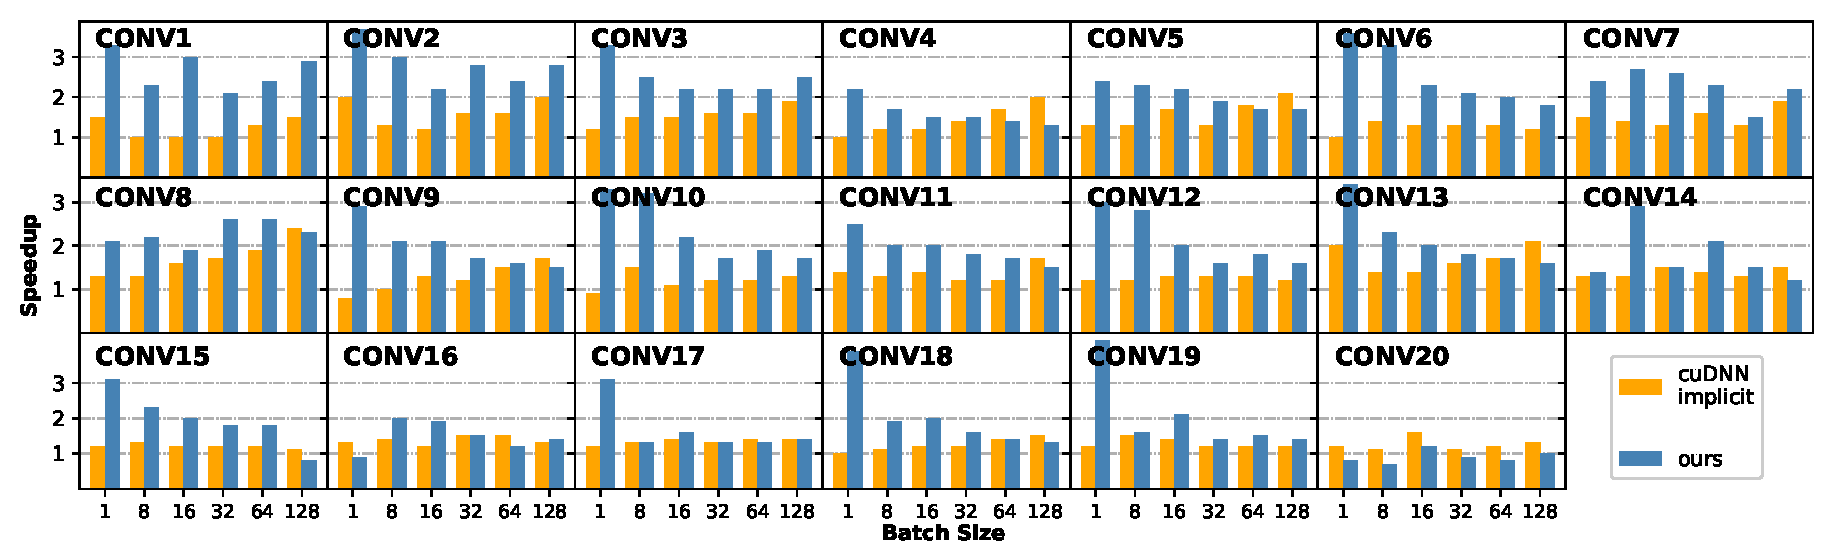
\includegraphics[width=\textwidth]{./figure/pwspeedupjetson.eps}
	\label{fig:pwspeedupjetson}}
	\vspace{-6mm}
	\caption{\RV{Speedups of IMPLICIT, PRECOMP and ours over GEMM for pointwise convolutions with FP32 on 2080Ti (top) and Xavier (bottom).}}
	\label{fig:pwspeedupfp32}
\end{figure*}

\begin{figure*}
\captionsetup[subfloat]{labelformat=empty,skip=0pt}

	\centering
	\subfloat[]{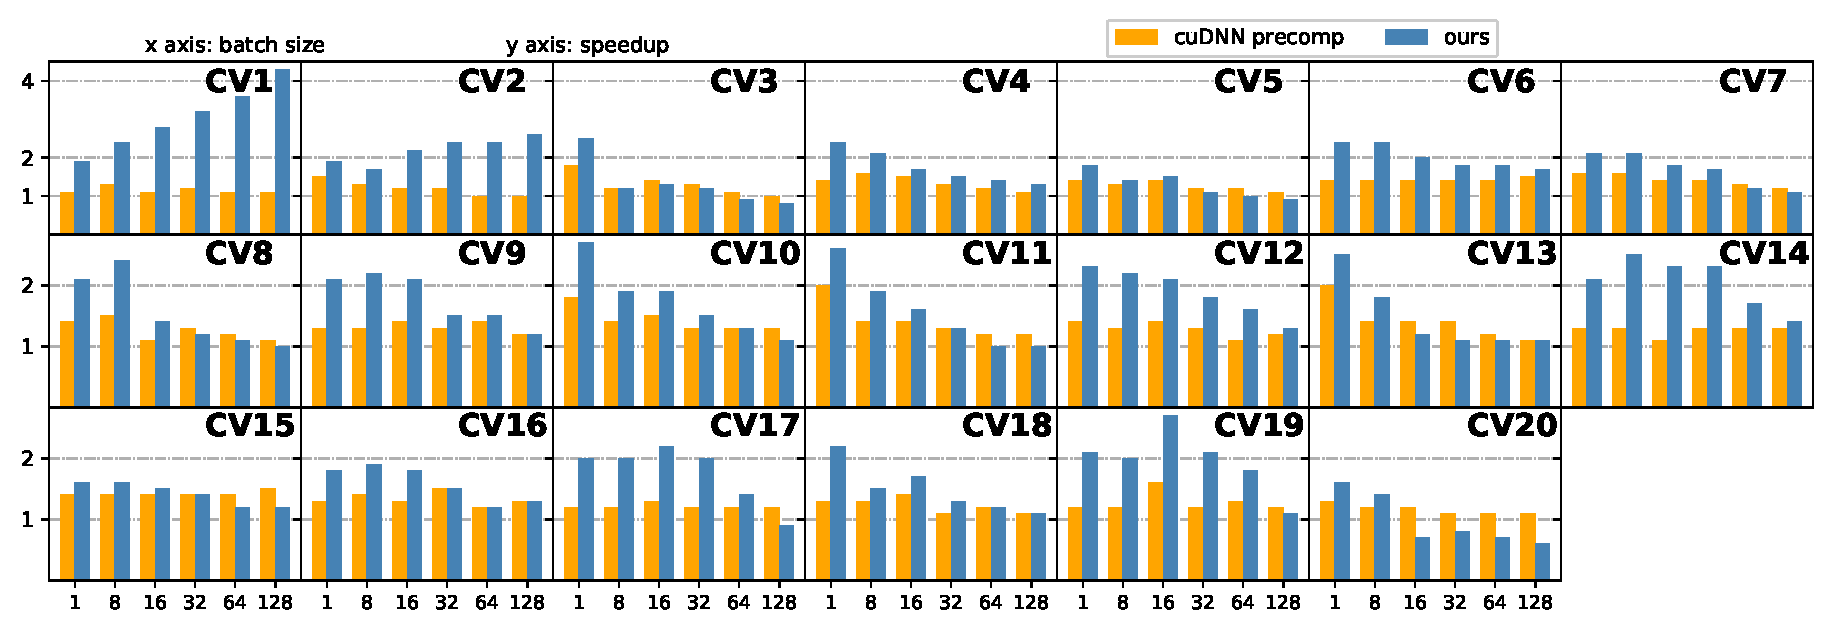
\includegraphics[width=\textwidth]{./figure/pwspeeduprtxint8.eps}
	\label{fig:pwspeeduprtxint8}}
	\vspace{-5mm}
	\subfloat[]{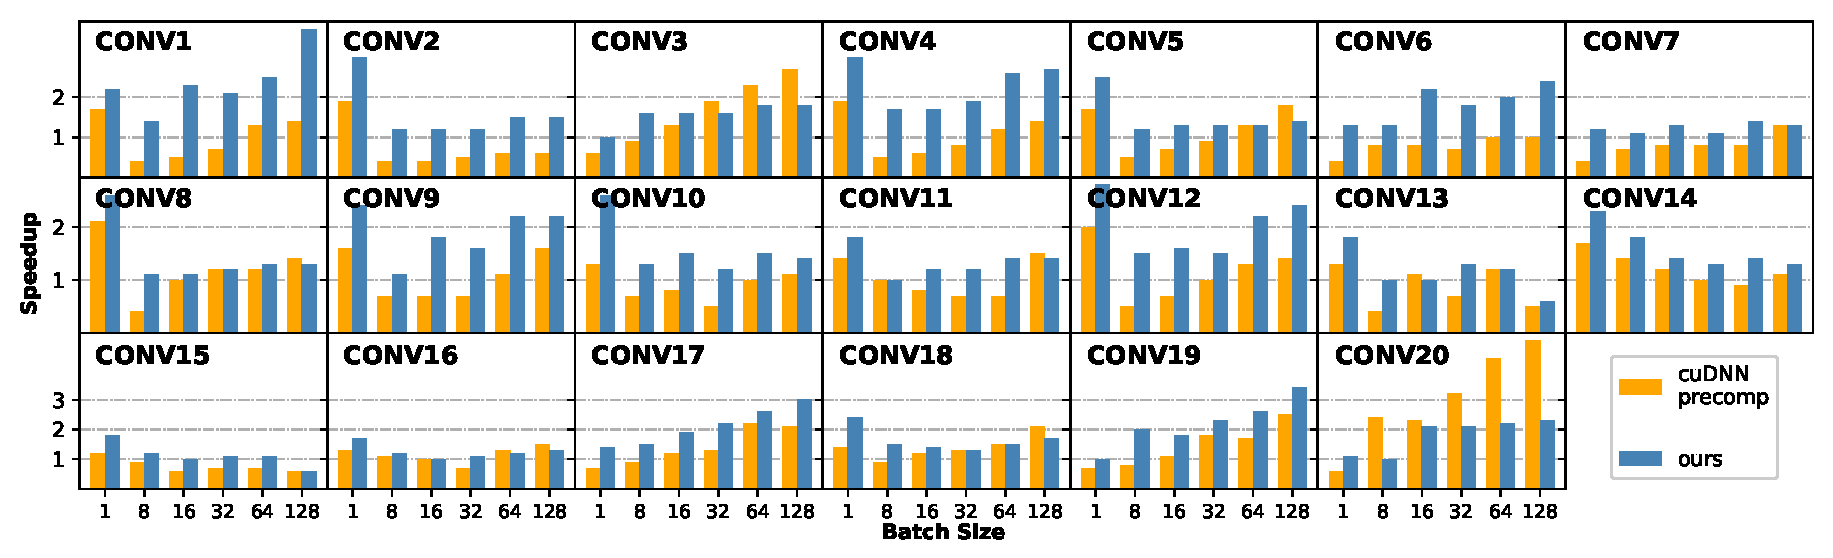
\includegraphics[width=\textwidth]{./figure/pwspeedupjetsonint8.eps}
	\label{fig:pwspeedupjetsonint8}}
	\vspace{-6mm}
	\caption{Speedups of PRECOMP and ours over IMPLICIT for pointwise convolutions with INT8 on 2080Ti (top) and Xavier (bottom).}
	\label{fig:pwspeedupint8}
\end{figure*}


\subsubsection{Setup} In this experiment, \RV{TensorFlow uses cuDNN implementations as their backend. Therefore, we only} compare our approach against all available pointwise convolution implementations in cuDNN.
The reported execution time of our approach includes the code running on both the CPU and the GPU, as described in Algorithm
\ref{algo:pwalgo}. We use the layer configurations from MobileNetV2 and EfficientNet-B0 in this experiment. Across different layers of the MobileNetV2 and EfficientNet-B0
models, there are 30 different configurations for pointwise convolution. We test all these configurations and report the performance of 20
selected layers. The other 10 layers exhibit similar performance as the selected ones and hence are omitted for clarity. We report the
performance when batch sizes are set to 1, 8, 16, 32, 64 and 128.

\RV{To aid clarify, we compare our approach to the best-performing alternative scheme - IMPLICIT and PRECOMP for FP32 and PRECOMP for INT8. When
using data type INT8, PRECOMP performs better than IMPLICIT in 180 out of 180 test cases on 2080Ti and 127 out of 180 test cases on
Xavier. For FP32, we normalize the speedup over GEMM. For INT8, because GEMM does not support this data type, we show the
speedup over IMPLICIT.} Table \ref{tab:pwconvandparas} lists the layer configurations \RV{and parameter values generated for
$Warp_H$, $Warp_W$, $Block_{num}$ and $C_{num}$ ($Warp_{num}=4$).} The notations can be found at Section \ref{sec:roadmap}.

\RV{Normally, for a given convolution layer configuration, when the width of the logical layout of the output (Fig. \ref{fig:pwworkflow}) is
small, our scheme tends to choose a small $C_{num}$. This allows one to generate more warps to utilize the GPU. On the other hand, our
scheme tends to choose a large $C_{num}$ to reduce the number of warps because there are already enough warps to maximize the utilization
of the GPU. A special parameter tuple (we take parameter tuples generated for 2080Ti as examples) is the layer configuration CONV9
with $I_N = 1$. The width of the logical layout of CONV9 is small. Hence we would like to search for a small $C_{num}$. However,
in this case, $C_{num} = 32$ is large. The reason is that our scheme finds that different values of $C_{num}$ gives similar GPU
utilization, then it tries to maximize AI (Formula \ref{fo:diff}) and then choose $C_{num} = 32$ (the relationship of AI and $C_{num}$ is
detailed in Section \ref{sec:cnum}). }

\subsubsection{Overall results}
\mypara{FP32 implementation.}  Fig. \ref{fig:pwspeedupfp32} shows speedups of IMPLICIT, PRECOMP and our approach for pointwise
convolutions on two platforms. The baseline is GEMM. 
%Our approach achieves the best performance for all layers except for CONV20
%where our approach gives modest slowdown over IMPLICIT and PRECOMP. This large convolution layer uses 1024 filters to convolve the
%input. Both cuDNN and our approaches are able to generate sufficient thread blocks to utilize the GPU cores. Under such scenarios, the
%memory access latency becomes the dominant bottleneck. The heavily optimized cuDNN enjoys the assembly level memory optimization to hide the
%goal memory access latency (as shown in Fig. \ref{fig:stalllongscore}), leading to better performance than our approach. Our approach can
%be further improved by employing a similar low-level optimization scheme. 
\RV{Average speedups of IMPLICIT, PRECOMP and our approach on 2080Ti and Xavier are shown in Table \ref{tab:pwspeedups}. The performance delivered by our approach translates to an improvement of $2\times$ and $1.5\times$ over IMPLICIT on 2080Ti and Xavier respectively.}

\begin{table}[]
\setlength{\tabcolsep}{2.5pt}
\caption{\RV{Average speedups of three pointwise convolution implementations over GEMM and IMPLICIT for FP32 and INT8 respectively.}}
\vspace{-3mm}
\label{tab:pwspeedups}
\centering
\rowcolors{2}{}{Gray}
\begin{threeparttable}
\begin{tabular}{l|r|r|r|r}
\toprule
& FP32, 2080Ti & FP32, Xavier &INT8, 2080Ti&INT8, Xavier\\
\midrule
IMPLICIT & 1.5 & 1.3 & 1.0 & 1.0\\
PRECOMP  & 1.3 & 1.1 & 1.3 & 1.2\\
ours     & 3.0 & 2.0 & 1.7 & 1.6\\
\bottomrule
\end{tabular}
\end{threeparttable}
\end{table}



\mypara{INT8 implementation.}  Fig. \ref{fig:pwspeedupint8} shows speedups of PRECOMP and our approach over IMPLICIT for
pointwise convolution. Table \ref{tab:pwspeedups} presents average speedups of PRECOMP and our approach over IMPLICIT on 2080Ti and Xavier. Overall, our approach obtains $1.3\times$ and $1.5\times$ improvement over PRECOMP on 2080Ti and Xavier respectively.


\subsubsection{Further analysis}
\begin{figure}[t!]
    \centering
    \subfloat[][SM utilizations of IMPLICIT and our approach.]{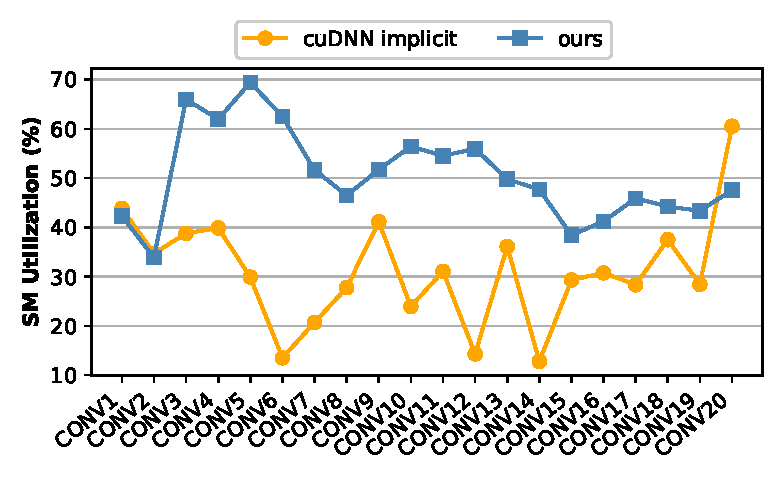
\includegraphics[width=\columnwidth]{./figure/pwsmutil.eps}\label{fig:pwsmutil}}
    \qquad

    \subfloat[][Ratios of executed LDG (load from global memory) instruction counts of IMPLICIT to our approach ($ratio=\frac{LDG\ inst\ counts\ of\ cuDNN}{LDG\ inst\ counts\ of\ ours}$).]{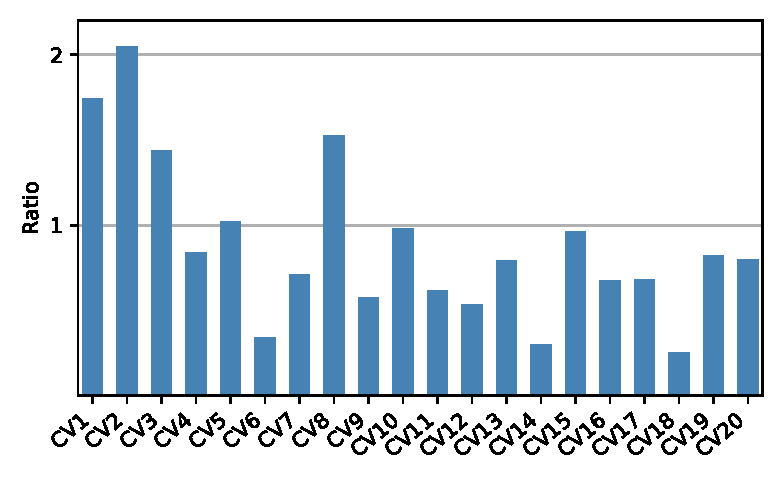
\includegraphics[width=\columnwidth]{./figure/pwldginst.eps}\label{fig:pwldginst}}
    \vspace{-2mm}
    \caption{SM utilizations and ratios of executed LDG instruction counts for pointwise convolutions with a batch size of 32 on 2080Ti.}
    \label{fig:pwinfo}
\end{figure}

\begin{figure*}[t!]
    \centering
    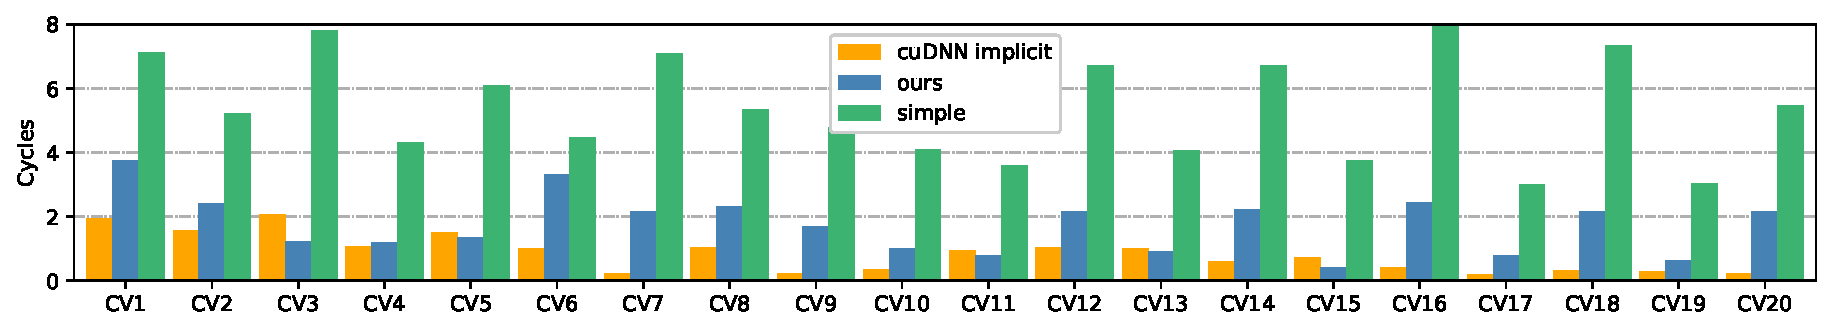
\includegraphics[width=0.97\textwidth,height=3cm]{./figure/longscore.eps}
    \vspace{-3mm}
    \caption{The average number of cycles each warp spends on waiting for the global memory access to complete.}
    \label{fig:stalllongscore}
\end{figure*}

Fig. \ref{fig:pwinfo} reports the measured SM utilizations and ratios of executed LDG instruction counts of IMPLICIT to our approach when using a batch size of 32 on 2080Ti. Other configurations have a similar performance.


For a specific layer configuration, our approach tries to find a suitable number of thread blocks to utilize the GPU. While using a higher
number of thread blocks can improve the GPU utilization, doing so can also incur frequent reloads of filters or inputs shared between
thread blocks. As shown in Fig. \ref{fig:pwldginst}, our approach leads to $2\times$ more LDG instructions than IMPLICIT in some
cases. Although using more LDG instructions incurs extra memory load overhead, our approach still gives $2\times$ faster execution time
over IMPLICIT due to our schemes for improving the SM utilization and hiding memory, elaborating as follows.


Our approach exhibits a much higher SM utilization than IMPLICIT. Unlike depthwise convolution, improving SM utilization is key for
optimizing pointwise convolution because utilizing more SMs can significantly accelerate the computation.	As can be seen from Fig.
\ref{fig:pwsmutil}, our approach has an average of $1.9\times$ higher SM utilization compared to IMPLICIT. IMPLICIT is
optimized for training and large batch-sized inference. It uses a fixed tile size work distribution strategy, which fails to utilize SMs
efficiently when using a batch size of 128 or smaller. Our dynamic tile size scheme (Section \ref{sec:pwinputdependent}) overcomes this
limitation by adaptively determining the right tile size to use at runtime, which thus leads to better SM utilization and performance improvement.

To hide the global memory access latency, our approach employs double buffering and channel distribution techniques as described in
Section \ref{sec:pwinputindependent}. To quantify the benefit of our memory optimization strategies, consider now  Fig. \ref{fig:stalllongscore} that
shows the average number of cycles each GPU warp spends on waiting for the GPU global memory access operation to complete. As a baseline,
we implemented a simple pointwise without latency hiding, denoted as simple. We can see that our approach can significantly reduce the
memory access latency compared to the simple implementation. Therefore, although our approach incurs a larger number of LDG instructions,
much of the memory access overhead can be hidden by our memory optimization strategy.



Furthermore, we observe some performance degradation for pointwise convolutions with the INT8 data type. When performing pointwise
convolutions with INT8, we use $NHWC$ data format, and four continuous INT8 channels can be viewed as an INT32 channel. Thus, the size of
the channel dimension is reduced to one-fourth of the original size. For small channel sizes ($I_C \leq 96$), the corresponding reduced channel
sizes restrict choices of the number of channels distributed, which leads to suboptimal performance compared to original channel sizes.
This can be improved by having a better channel size allocation scheme for INT8. We leave this as our future work.

\RV{From Figs. \ref{fig:pwspeedupfp32} and \ref{fig:pwspeedupint8}, we see that our approach is more noticeable on small batch sizes. This
is because that pointwise convolution is more sensitive to the GPU utilization. A larger batch size tends to use more warps, which alone can improve the GPU utilization and further improve the performance of cuDNN. For example, the speedups of our approach over cuDNN when $I_N=128$ are much smaller than the speedups when $I_N<128$. By contrast, when the batch size is smaller, the resulting warps alone is insufficient in utilizing the GPU
where our dynamic tile size scheme can help. }

\subsubsection{Summary} Our approach uses a dynamic tile size method to improve SM utilization and double-buffering and channel distribution to hide
memory access latency. With the help of both methods, we achieve an average speedup of $2\times$ and $1.5\times$ over IMPLICIT on
2080Ti and Xavier, respectively.





\subsection{End to End Performance for Inference and Training}
\label{sec:inferexp}
\subsubsection{Setup}
In this experiment, we apply our depthwise and pointwise convolutions to MobileNetV2 and EfficientNet-B0 and report the end-to-end performance of inference and training \RV{with ImageNet dataset \cite{deng2009imagenet}}.

\mypara{Inference.} For inference, we test standard and quantized MobileNetV2 and EfficientNet-B0 with batch sizes of 1, 8, 16, 32, 64 and 128 on both
platforms and report the respective inference time. For quantization, the input and filter are converting from FP32 to INT8, and the
results are converted back to FP32 as the model output. As cuDNN performs poorly for depthwise convolutions with INT8, we do not apply
quantization to depthwise convolutions for fair comparisons.

\mypara{Training.} For training, we test MobileNetV2 and EfficientNet-B0 with batch sizes of 16, 32, 64 and 128 on 2080Ti and report the average training time
of one training iteration, including the forward and the back-propagation phases.

\mypara{Workload and performance report.} We use the open-source MobileNetV2 and EfficientNet-B0 implemented using the Caffe framework, but we replace the
implementations of batch normalization and depthwise convolution layers with the heavily optimized cuDNN implementations. The cuDNN
implementation is denoted as \textbf{cuDNN} and our implementation is denoted as \textbf{Ours}. We report the percentage of performance
improvement of our approach compared to cuDNN implementations, denoted as \textbf{Improved}.


\subsubsection{Overall results}
\begin{table*}[]
\setlength{\tabcolsep}{5.4pt}
    \caption{\RV{Inference time of MobileNetV2 and EfficientNet-B0 with FP32 and INT8 on 2080Ti and Xavier.}}
    \vspace{-3mm}
    \label{tab:infertime}
    \centering
    %\rowcolors{2}{}{Gray}
    \begin{threeparttable}
    \begin{tabular}{c|l|rrrrrr|rrrrrr}
    \toprule
    \multicolumn{2}{c|}{} & \multicolumn{6}{c|}{MobileNetV2} & \multicolumn{6}{c}{EfficientNet-B0}\\
    \midrule
    &\textbf{Batch} & 1 & 8 & 16& 32 &64 & 128& 1 & 8 & 16& 32 &64 & 128\\
    \midrule
    %normal MobileNetV2
    \multirow{3}{*}{\textbf{\shortstack{2080Ti\\(FP32)}}}&\textbf{cuDNN (ms)}   &7.5  &8.8  &9.7  &14.4 &19.1 &28.7 &10.1&13.7&18.1&25.0&36.4&52.3\\
    &\textbf{Ours (ms)}    &6.1  &7.1  &8.0  &12.0 &16.9 &26.3&7.9&11.3&15.3&21.9&32.6&47.6\\
    &\textbf{Improved (\%)} &18.6 &19.3 &17.5 &16.7 &11.5 &8.4&21.8&17.5&15.5&12.4&10.4&9.0 \\
    \hline
    \multirow{3}{*}{\textbf{\shortstack{Xavier\\(FP32)}}}&\textbf{cuDNN (ms)}   &16.6 &22.3 &32.1 &52.6 &84.2 &140.1&19.3&27.4&38.3&57.2&94.0&157.8  \\
    &\textbf{Ours (ms)}    &13.2 &18.9 &27.8 &44.7 &76.1 &130.0&15.5&23.2&32.1&50.7&87.3&151.1 \\
    &\textbf{Improve (\%)} &20.5 &15.2 &13.4 &15.0 &9.6  &7.2&19.7&15.3&16.3&11.4&7.1&4.2 \\
    \hline
    %quantized MobileNetV2
    \multirow{3}{*}{\textbf{\shortstack{2080Ti\\(INT8)}}}
    &\textbf{cuDNN (ms)}   &6.3  &7.4  &7.7  &11.2 &14.6 &20.2&8.0&9.5&13.3&18.7&26.8&38.3 \\
    &\textbf{Ours (ms)}    &5.5  &6.6  &6.8  &10.3 &14.0 &19.7&6.8&8.2&11.8&16.9&25.3&36.6\\
    &\textbf{Improved (\%)} &12.7 &10.8 &11.7 &8.0  &4.1  &2.5&15.0&13.7&11.3&9.6&5.6&4.4 \\
    \hline
    \multirow{3}{*}{\textbf{\shortstack{Xavier\\(INT8)}}}
    &\textbf{cuDNN (ms)}   &13.3 &18.0 &27.0 &42.6 &64.8 &103.7&16.1&21.0&33.7&52.8&80.3&127.5  \\
    &\textbf{Ours (ms)}    &11.7 &15.4 &22.7 &38.8 &58.3 &94.4&14.2&18.8&30.3&48.2&73.2&117.7 \\
    &\textbf{Improved (\%)} &12.0 &14.4 &16.0 &8.9 &10.0  &9.0&11.8&10.5&10.1&8.7&8.8&7.7 \\


    \bottomrule
    \end{tabular}
    \footnotesize
    \end{threeparttable}

\end{table*}

\begin{table}[]
\setlength{\tabcolsep}{4.4pt}
    \caption{\RV{Training time of MobileNetV2 and EfficientNet-B0 with FP32 on 2080Ti.}}
    \vspace{-3mm}
    \label{tab:traintime}
    \centering
    %\rowcolors{2}{}{Gray}
    \begin{threeparttable}
    \begin{tabular}{l|rrrr|rrrr}
    \toprule
    &\multicolumn{4}{c|}{MobileNetV2} & \multicolumn{4}{c}{EfficientNet-B0}\\
    \midrule
    %\hline
    \textbf{Batch} & 16& 32 &64 & 128& 16& 32 &64 & 128\\
    \midrule
    %\hline
    \textbf{cuDNN (ms)} & 16.6 & 27.6 & 43,4 &75.4& 33.5 & 49.3 & 74.7 &116.2 \\
    \textbf{Ours (ms)} & 14.5  &24.1 &39.9 &71.3& 30.0  &45.1 &69.6 &112.4\\
    \textbf{Improved (\%)} &12.7  &12.7 &8.1 &5.4 &10.4  &8.5 &6.8 &3.3\\
    \bottomrule
    \end{tabular}
    \footnotesize
    \end{threeparttable}
    \vspace{-5mm}
\end{table}

Table \ref{tab:infertime} reports the measured inference time. For MobileNetV2 with FP32, our approach improves the performance of
inference by 12.2\% and 13.5\% on average compared to IMPLICIT on 2080Ti and Xavier, respectively. For MobileNetV2 with INT8, we
obtain 8.5\% and 11.7\% improvements on average over PRECOMP on 2080Ti and Xavier, respectively. \RV{For EfficientNet-B0 with FP32, our approach improves IMPLICIT by 14.4\% and 12.3\% on average on 2080Ti and Xavier, respectively. For EfficientNet-B0 with INT8, we obtain 9.9\% and 9.6\% improvements on average over PRECOMP on 2080Ti and Xavier, respectively.}
Table \ref{tab:traintime} shows that
our approach averagely reduces the training time of MobileNetV2 and EfficientNet-B0 by 9.7\% and 7.3\% compared to IMPLICIT on 2080Ti, respectively. The results show that our approach can
significantly reduce both the model inference and training time by speeding up DSC operations.
